\section{Introducing \pace: Pullback Averaging Control for Efficient Optimization}
\label{sec:method}

\begin{figure}[t]
    \centering
    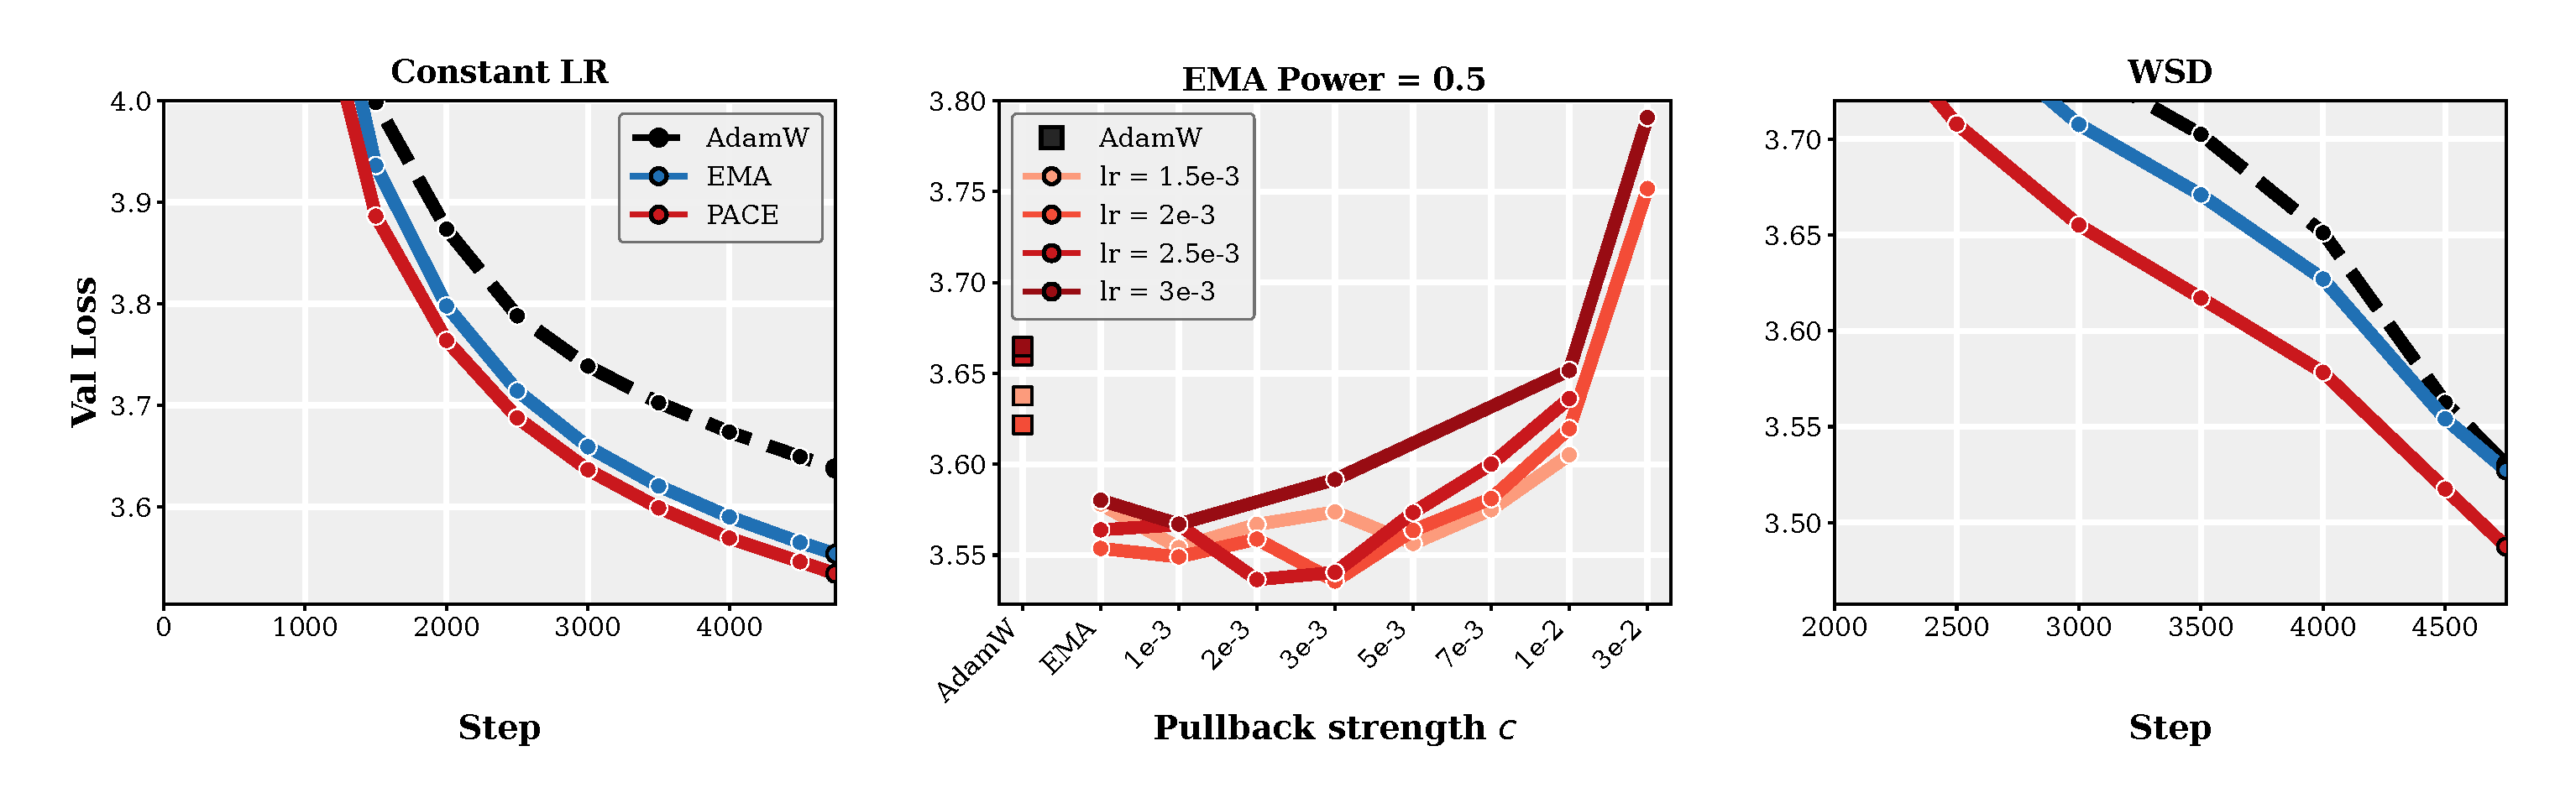
\includegraphics[width=\textwidth]{figures/fig5_pretraining.pdf}
    \caption{
        \textbf{Performance of \pace\ on pretraining} of GPT-2 (124M) on FineWeb at the Chinchilla-optimal token budget. \textbf{Left:} validation cross-entropy trajectories at a constant learning rate, with \ema\ and \pace\ at the same EMA power ($\kappa=0.5$) so that they differ only in the pullback. \textbf{Middle:} effect of pullback strength $c$ on validation cross-entropy at $\kappa=0.5$. \textbf{Right:} the analogous comparison under WSD, using linear learning rate decay to zero over the last $20\%$ of steps. \pace\ outperforms both the AdamW and \ema\ baselines under each schedule.
    }
    \label{fig:pretrain}
\end{figure}

While we derived a simple modification to the base optimization algorithm in \eqref{eq:stylized_update}, several additional tweaks make the proposed method work in practice.  The first key modification is that we will replace the SGD update with an AdamW update \citep{loshchilov2017fixing}, which is a standard optimizer choice for language models; in particular, we will use both momentum and preconditioning in the vanilla optimizer step.  The second question is how to choose the matrix $\bC$ that preconditions the pullback toward the iterate average.  According to the theory in \eqref{eq:practical_control_strategy}, the optimal choice of $\bC$ scales inversely with $\bA$ and $T$.  While in practice language models are obviously not quadratic, locally they can be approximated thereby, with $\bA$ corresponding to the Hessian \citep{zhang2019algorithmic,zhang2019lookahead}; following the standard noisy-quadratic-model identification of Adam's second-moment estimate $v_t$ as a Hessian-diagonal proxy, we will thus set $\bC$ to be a diagonal matrix with entries given by the Adam preconditioner \citep{kingma2014adam}.  One point where our empirical implementation deviates from the theory is that the latter suggests preconditioning should be scale like $\nicefrac 1{v_t}$, but for stability reasons we find that the standard Adam preconditioner of $\nicefrac 1{\sqrt{v_t} + \varepsilon}$ works better in practice.  

Following standard praxis in deep learning, in order to account for the nonstationarity of the optimization landscape, we replace a fixed $\beta$ in the EMA with a decaying $\beta_t = (1+t)^{-\kappa}$, where $\kappa \in (0, 1)$ is a hyperparameter \citep{busbridge2023scale,block2025ema,block2024butterfly,kaddour2022stop}; in effect this makes the iterate average more responsive to recent iterates, with $\kappa = 1$ recovering uniform averaging.  For the same reason, we replace the $T^{-1}$ scaling in \eqref{eq:practical_control_strategy} with a slower decaying factor that allows the pullback to remain significant even late in training.  We incorporate clipping to ensure that our updates are always convex combinations of the iterate averaged point and the na{\"i}ve optimizer update step. The resulting control becomes
\begin{align}\label{eq:practical_control_strategy_empirical}
    u_{t} = \min\left( (1 + t)^{- \kappa} \cdot \nicefrac{\eta c}{\left( \sqrt{v_{t}} + \epsilon \right)}, 1 \right)\left( \thetema[t] - \theta_t \right),
\end{align}
where the operations are applied coordinate-wise, $\eta$ is the learning rate, $c \geq 0$ is a single scalar setting the controller strength, and $v_t$ is the Adam second-moment estimate.  Note that in the limit as $c \uparrow \infty$, we recover the Lookahead optimizer with an inner loop of a single step \citep{zhang2019lookahead}, while at $c=  0$, we recover AdamW with \ema.  Finally, we allow for the update to only occur at a specified frequency, $\mathrm{uf}$, as is common in practical implementations of \ema. The result, \pace, is detailed in \cref{alg:controlled-bema}.  

\paragraph{Implementation Concerns.} In practice, there are two concerns with implementing \pace\ at scale.  First, we have introduced a new tuning parameter $c$ that controls the strength of the pullback toward the iterate average, as well as the update frequency $\mathrm{uf}$; on the other hand, the update frequency is already a parameter in standard implementations of \ema, and our experiments suggest that the optimal pullback strength is relatively robust and transfers across hyperparameters like learning rate (cf. \Cref{fig:135m_grid}).
Second, and perhaps more importantly, \pace\ requires maintaining an additional copy of model weights during training, which is a nontrivial memory overhead.  One mitigating factor is that this additional pressure is less relevant at large scale due to the use of large batch sizes, but exploring further mitigations of the memory overhead of \pace\ is an important direction for future work.





\begin{figure}[t]
    \centering
    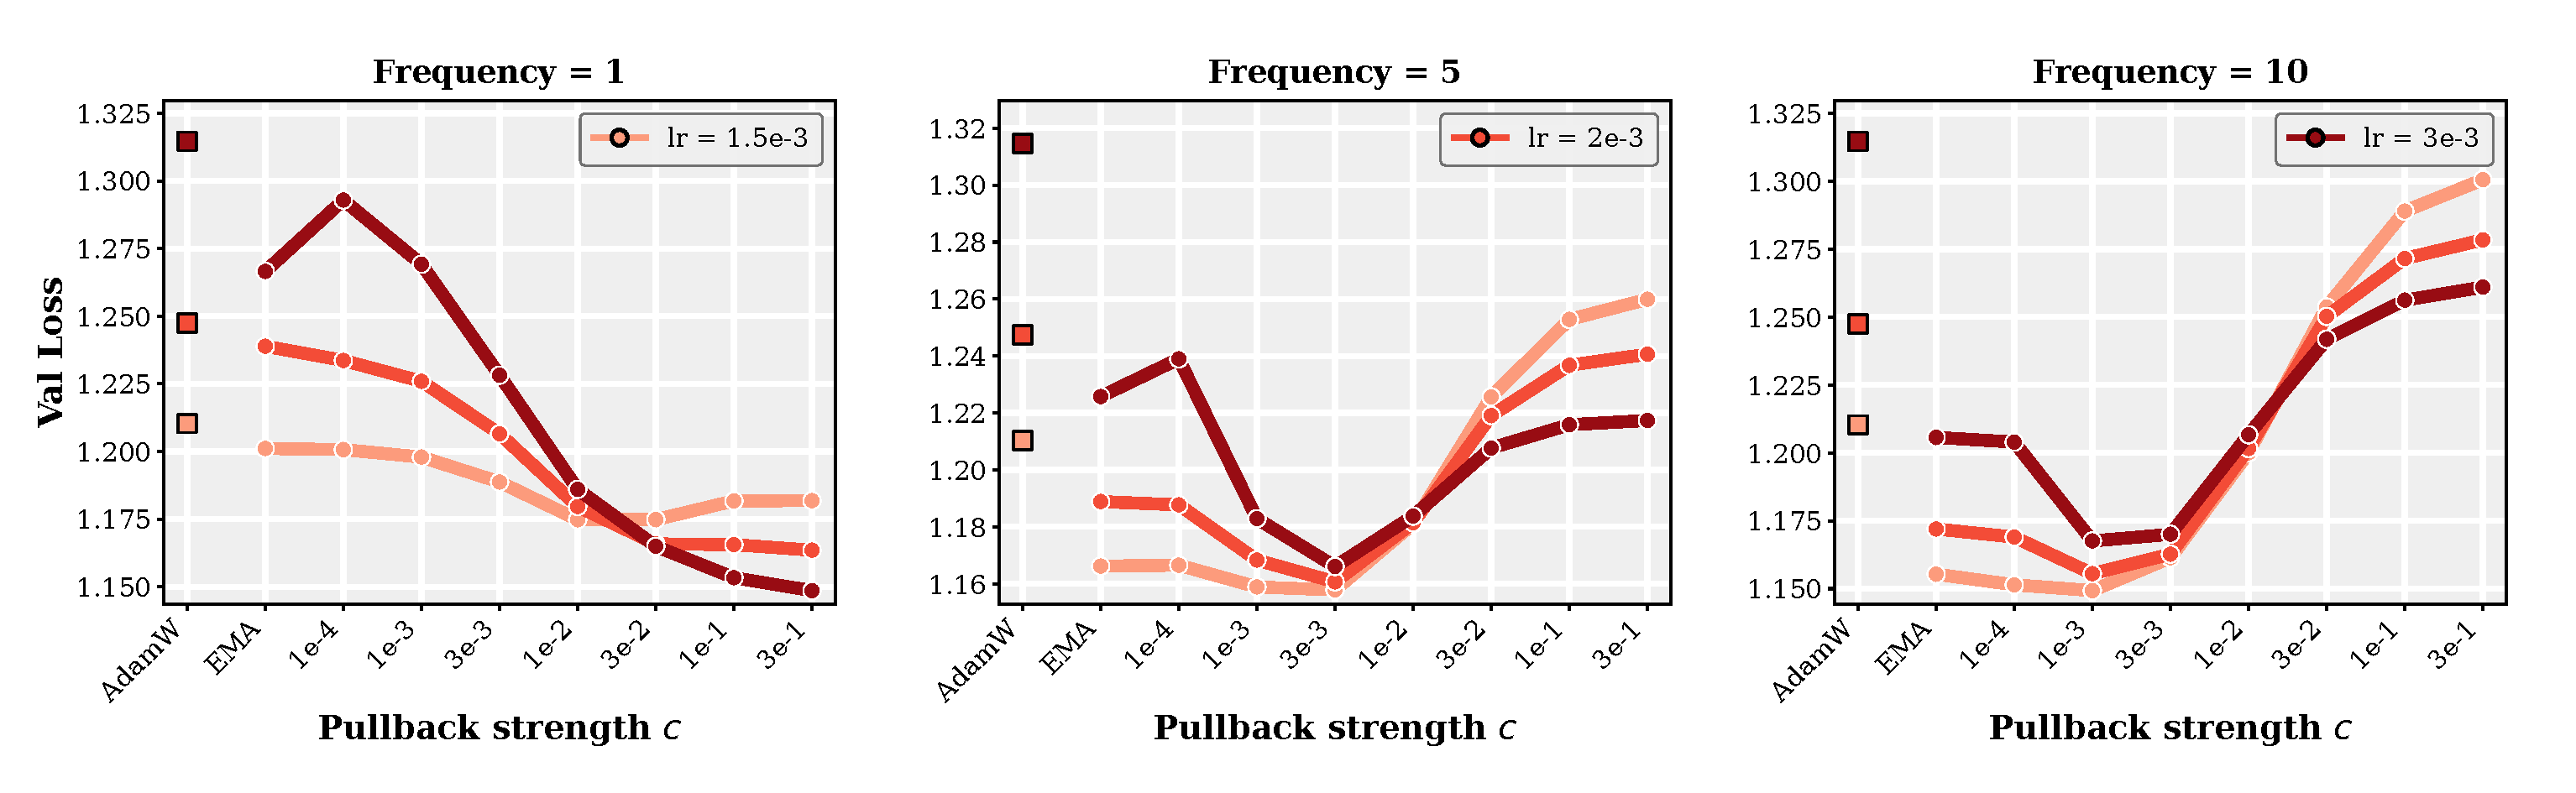
\includegraphics[width=\textwidth]{figures/fig3_135m_grid.pdf}
    \caption{\textbf{Effect of update frequency and pullback strength.} Validation cross-entropy of SmolLM2-135M for different learning rates, pullback strengths, and update frequencies with $\kappa{=}0.3$.  Optimal pullback strength remains relatively robust to learning rate and update frequency, with improvement over the EMA baseline across a wide range of settings.}
    \label{fig:135m_grid}
\end{figure}


